\chapter{Design \& Methodology}
\label{chapter:design}

This chapter will detail the methodology used for the duration of this project, including the software development process and the project management system. This chapter will also provide a detailed look into the design of each component of the system, including the decisions behind each design choice based on the research that was discussed in chapter \ref{chapter:research}.

\section{Methodology}
A Scrum-like software development methodology was used for the duration of this project, along with elements from the Kanban method.

Scrum is a kind of Agile development methodology that is based on a series of iterative cycles of development called \emph{sprints}. These sprints will often begin with a brief planning session, can last from 1 to 4 weeks, then finish with a sprint retrospective to review how it went.

% todo: ref scrum
% todo: Fix tenses in this section

Scrum is usually a heavily team-based process, involving several roles such as `Scrum Master`, `Product Owner' and the Scrum team. Daily 15 minute team meetings are held to assess how the sprint is going, with each role and team member talking about what they did and what they plan to do. Since this project will be completed by a single person, I will be focusing on the iterative development, planning and review aspects of the Scrum methodology rather than the daily meetings and roles.

% todo: http://www.mountaingoatsoftware.com/agile/scrum

Using an Agile methodology like Scrum means that most of the design of the application will be done as needed, rather than up front such as in the waterfall model. Design documents such as entity-relationship diagrams will be completed as they become necessary for the continuation of the development process, or if another part of the project depends on the design being completed.

\subsection{Project Management}
A \emph{kanban board} will be used to manage tasks during each sprint. Trello will be used as the board by adding a list for each iteration in the development process. Cards will be added to these lists for each task, and labels will be used as kanban columns by using labels such as `Ready', `In Progress', and `Completed' as can be seen in Figure \ref{fig:kanban}. If cards are overdue, they can be moved to the next sprint list as a backlog, by dragging and dropping.

% todo: Ref kanban

\begin{figure}[h]
	\centering
	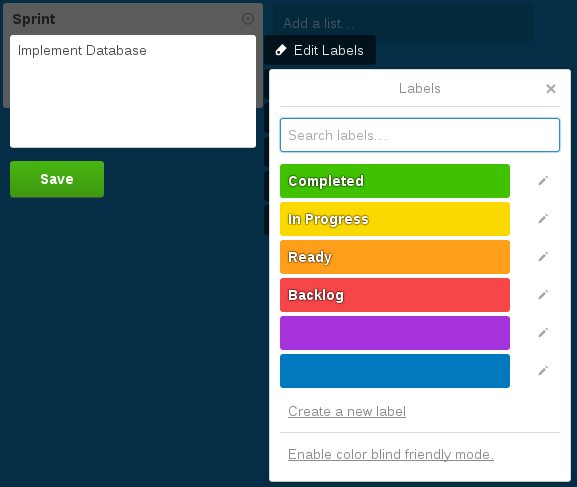
\includegraphics[scale=0.7]{kanban}
	\caption{Kanban-style task labels in Trello}
	\label{fig:kanban}
\end{figure}

%todo: fix branching

Git will be used throughout the development process to provide version control and project management through branches. Branching will be used to manage the status of the project via stable and development branches. The Git repository will be hosted both locally and remotely on GitHub for a backup.

% todo git appendices - graphs?

\section{User Interface}
% Usability, how being on the web affected interface design
	\subsection{Website}
	The website will be what the user interacts with initially when they visit the web application, which is where they are able to browse games published by other users or manage their own games. Neilsen's heuristics were taken into consideration while designing this portion of the application, leaning strongly towards aesthetic and minimal design while creating the user interface.

	% todo ref Neilsen's Heuristics

	\paragraph{Horizontal Prototype.}
	In order to begin developing the website for this project, a medium fidelity horizontal prototype was created. The horizontal prototype allowed me to examine how the user would interact with the system, and visualise the actions that the user will perform while using it. This was also helpful for minimising potential usability problems later on.

	% todo ref

	% todo figures
	\begin{figure}[h]
		\centering
		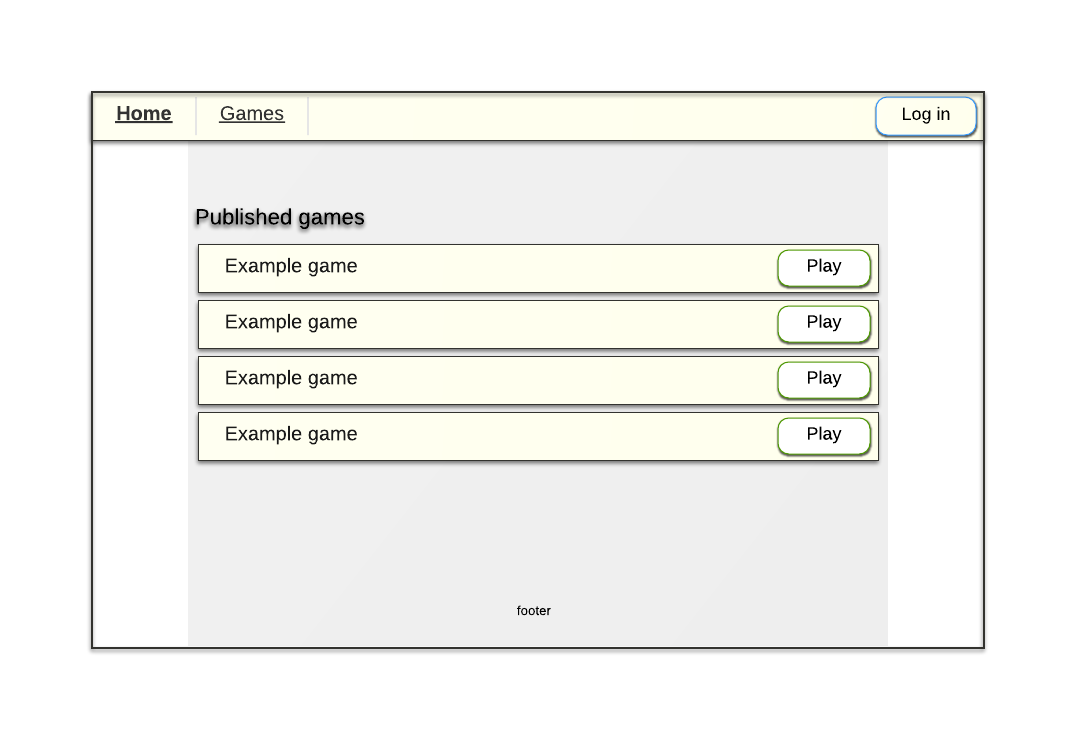
\includegraphics[scale=0.7]{websitehoz}
		\caption{Front page horizontal prototype}
		\label{fig:frontpageprototype}
	\end{figure}

	Figure \ref{fig:frontpageprototype} shows the horizontal prototype design for the front page of the website. This shows the actions available to a guest on the system; such as logging in, or browsing the games published by other users on the system. The user is able to click `Play' on one of the available games to launch into a new page where they can play that game.

	\begin{figure}[h]
		\centering
		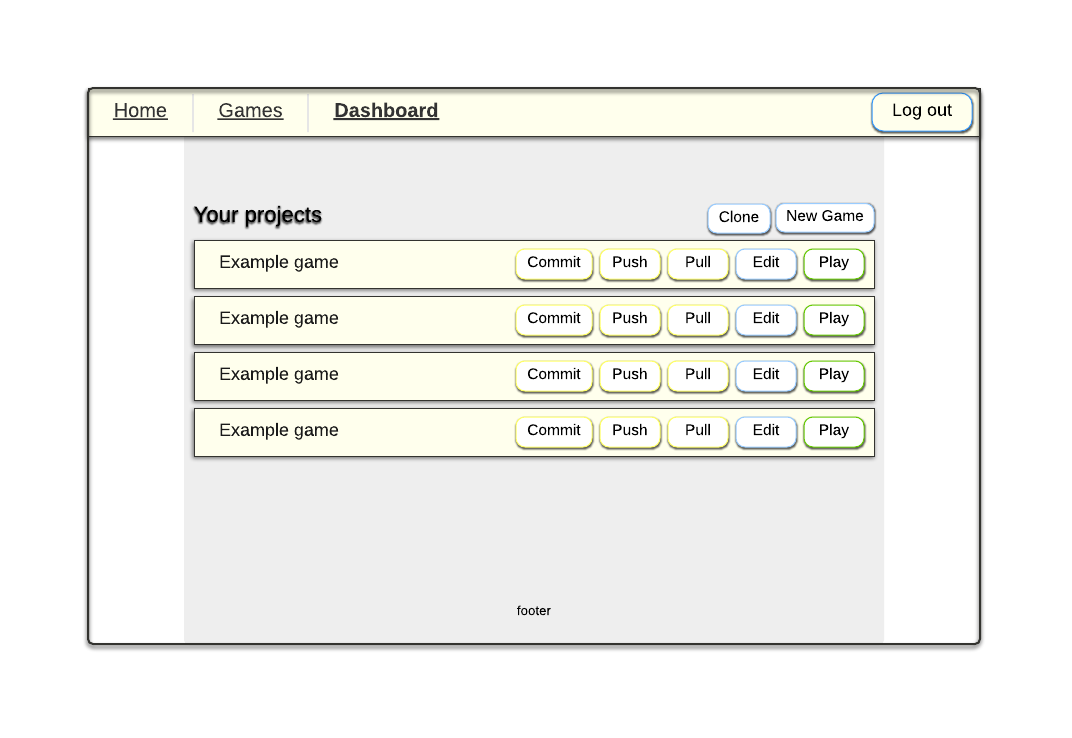
\includegraphics[scale=0.7]{dashboardhoz}
		\caption{Dashboard horizontal prototype}
		\label{fig:dashboardprototype}
	\end{figure}

	Figure \ref{fig:dashboardprototype} shows the design of the dashboard; where logged in users can manage their games on the system. The dashboard allows logged in users to add a new game project, delete an existing one, launch into the editor for a project, or playtest their game. There are also actions available to clone a repository from GitHub, make commits, and push \& pull an existing project to and from GitHub.

	\paragraph{Evaluation}
	These prototypes were evaluated using the IxD (Interaction Design) checklist; which is a checklist of usability, feedback, and accessibility functionality for analysing the usability of a system based on Neilsen's Heuristics. The `Interface' section of the checklist was selected, as the prototypes were only medium fidelity. By going through the checklist it was determined that the prototypes were suitable for use in the web application as they met 100\% of the criteria on the checklist.

	% todo: website

	% ref IxD

	\subsection{Game Editor}
	The game editor is the most important part of the website; this is where users will be able to construct scenes for their games by creating new scenes, entities and components. The interface for this part of the web application was designed to be similar in regards to the Unity game editor; as it provides a familiar experience for those who have used it. It was also designed with Neilsen's heuristics in mind, aiming for a high usability rating.

	% ref neilsen

	\paragraph{Horizontal Prototype.}
	The prototype for the game editor can be seen in Figure \ref{fig:gameeditorprototype}. The layout of the editor is split into three columns; the \emph{explorer}, \emph{scene view}, and \emph{properties}. There are also tabs that will contain a script editor, allowing the user to switch to it and create their own custom components.

	% todo fig
	\begin{figure}[h]
		\centering
		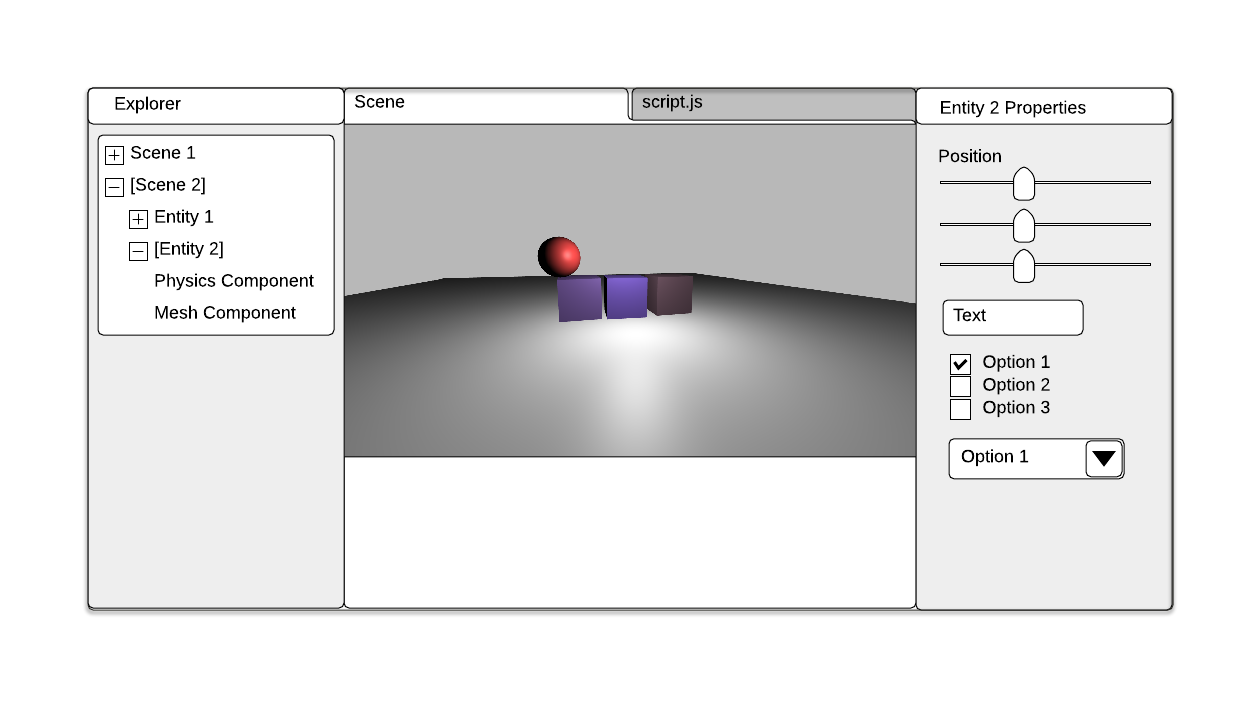
\includegraphics[scale=0.7]{editorhoz}
		\caption{Game editor horizontal prototype}
		\label{fig:gameeditorprototype}
	\end{figure}

	\paragraph{Explorer.}
	In the explorer, a tree of the current game is displayed, where scenes contain a list of entities, and entities contain a list of components. Actions can be performed on these scenes, entities and components such as adding, deleting or copying.

	\paragraph{Scene View.}
	The scene view is the centerpiece of the editor, which displays a visualisation of the currently selected scene along with all entities inside of it. The scene view updates realtime with any changes that are made in the editor, providing feedback to the user when they add, delete or change properties on an entity.

	\paragraph{Properties.}
	The properties list shows a list of the components and their respective properties for the selected entity in the explorer. Here the user will be able to change the properties of components on entities; such as colours, position, scale, and rotation. When property changes are made, the scene will update accordingly.

	\paragraph{Evaluation.}
	The evaluation of the editor horizontal prototype was also carried out using the IxD checklist, using the `Interface' section of the checklist. The result of filling in the checklist determined that the prototype design of the editor was suitable for the project, as it met 100\% of the criteria in the checklist.

	% ref IxD

\section{System Components}
There are several key components in this system that have been carefully designed to work together, with each component having it's own design. This section will look at the structure of these components and how they have been designed to work together.

	\subsection{Overview}
	The components of this system are the web server, storage server, MongoDB database, website, game engine and game editor. Figure \ref{fig:overalldesign} visualises these components and shows how they interact with eachother, and what the user accesses.

	\begin{figure}[h]
		\centering
		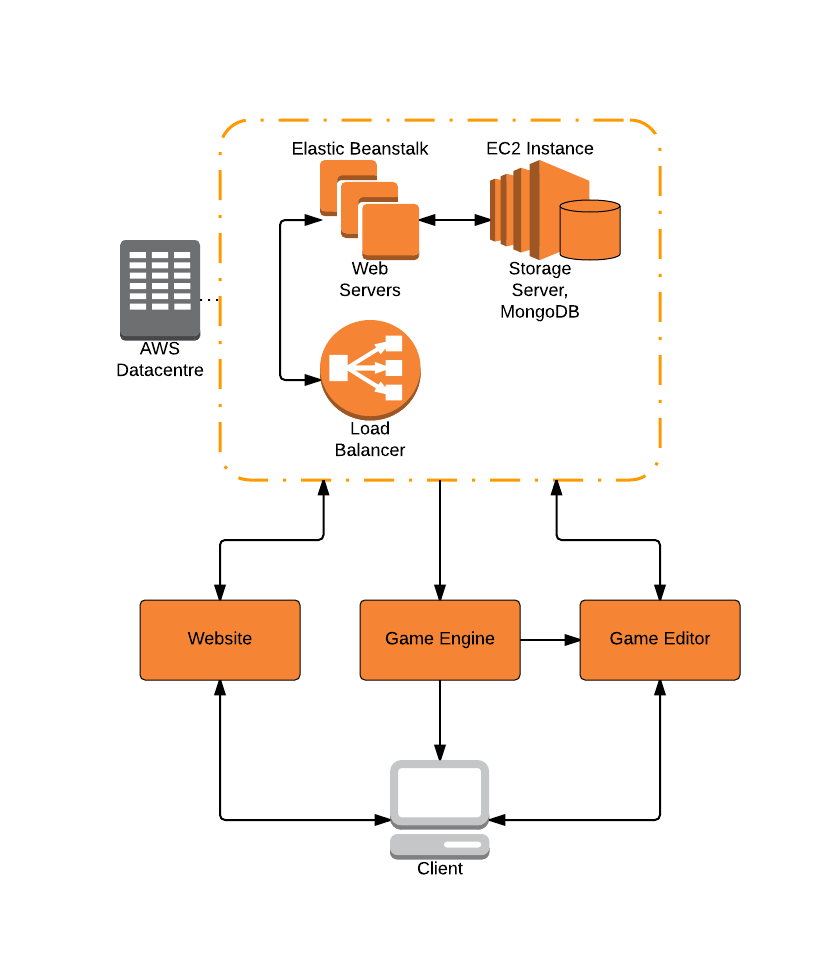
\includegraphics[scale=0.6]{overalldesign}
		\caption{System components overview}
		\label{fig:overalldesign}
	\end{figure}

	Clients connect to the web application through the load balancer to view either the website, a game, or the game editor. When the connection to the load balancer is initiated, the load balancer can create a new instance of the web server if needed, to allow automatic scaling. The web servers will communicate with the storage server to retrieve or store game projects that have been created by users. The MongoDB database, which runs on the same system as the storage server, is used to store a list of games published by the users.

	\paragraph{Network}
	%ec2, beanstalk
	The network of the system has been designed to prevent access to the storage server to normal users. Any request to store or retrieve a user's project goes through the a web server instance, which requires the client be logged in if they want to make any changes. For this purpose, the storage server is assigned a security group on Amazon VPC (Virtual Private Cloud) to allow TCP connections only from the local subnet. This means that any user trying to connect to the storage server directly will not be able to connect. This system can be seen in Figure \ref{fig:awsnetworkdesign}.
	% todo ref VPC, security groups, load balancer?

	\begin{figure}[h]
		\centering
		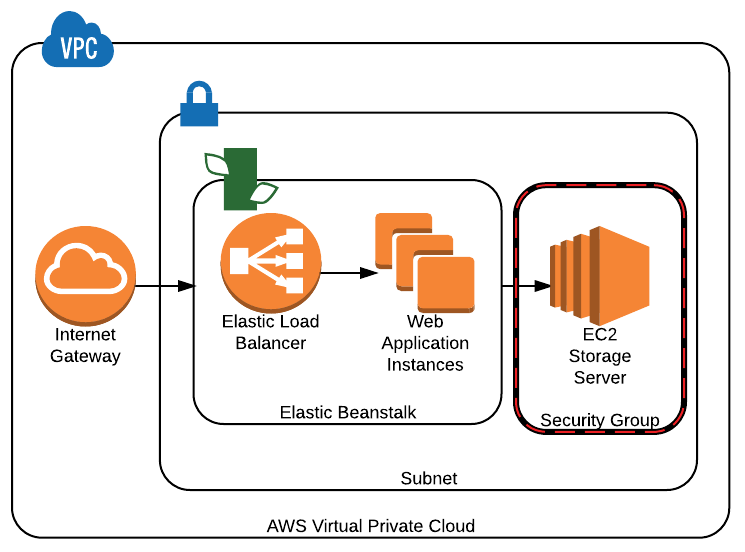
\includegraphics[scale=1.0]{awsdesign}
		\caption{AWS network design}
		\label{fig:awsnetworkdesign}
	\end{figure}

	The network is also designed around scalability, with load balancing being the main focus. Any connection to the web application goes through the load balancer, which can create multiple instances of the web application as needed. Because multiple web applications are created, it was important to centralise the storage of the users' projects in a separate server, which could be used by all application instances.

	\subsection{Storage Server}
	\label{subsection:storageserverdesign}
	% ec2
	The storage server is designed as a fairly simple REST API built with Flask, which allows actions based on the HTTP request type. For example, a HTTP \emph{GET} request will \textbf{return} a resource, a \emph{POST} request will \textbf{create} a resource, and \emph{DELETE} will \emph{delete} one. This provides a very simple interface over the web for controlling resources on a server, especially around a filesystem.

	% todo ref RESTful
	The storage server will be deployed on an Amazon EC2 (Elastic Compute Cloud) instance, with a mounted Elastic Block Storage drive. The server will store user projects in the EBS filesystem in a tree structure, in which each user will have their own folder containing a folder for each of their projects. The API is designed around this, with the RESTful commands taking a form such as:

	GET /<user>/<repo>/file/game.json

	\paragraph{API.}
	The API provides several methods for controlling the resources of projects on the storage server, such as retrieving information, performing Git operations, and retrieving \& storing files. The routes below were designed to provide a very strong API backend for storing projects.

	\begin{itemize}
		\item GET - Retrieve information:
		\begin{itemize}
			\item /<user>
			\item /<user>/<repo>/status
			\item /<user>/<repo>/tree/<path>
		\end{itemize}
		\item POST - Perform action:
		\begin{itemize}
			\item /<user>/<repo>/push/<remote>
			\item /<user>/<repo>/pull/<remote>
			\item /<user>/<repo>/commit
		\end{itemize}
		\item GET/PUT/POST/DELETE - Control resource:
		\begin{itemize}
			\item /<user>/<repo>
			\item /<user>/<repo>/file/<path>
		\end{itemize}
	\end{itemize}

	\paragraph{GitPython.}
	The storage server utilises a Python library called GitPython to perform Git operations on the users' game project folders. This provides a much better method for performing the Git operations than using the GitHub API for committing and pushing any changes to the users' game projects. Operations such as performing a commit are near instant; as it's only modifying local files, whereas they could take up to 10 seconds using the GitHub API; which requires multiple requests for a single commit.

	\subsection{MongoDB}
	To provide the web application with a method of keeping track of published games, a MongoDB server will be set up on the EC2 instance running the storage server. The simple NoSQL structure of MongoDB allows for a very lightweight document design to be used for storing the published game details as seen in Figure \ref{fig:nosqldesign}.

	% todo ref mongodb

	\begin{figure}[h]
		\centering
		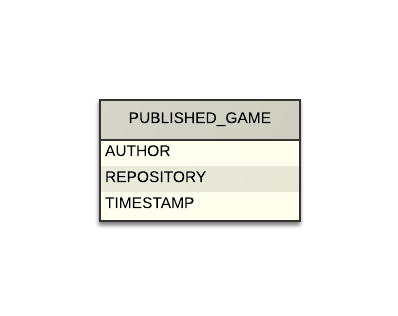
\includegraphics[scale=0.8]{nosqldesign}
		\caption{MongoDB document design}
		\label{fig:nosqldesign}
	\end{figure}

	\subsection{Web Server}
	The web server is a key part of the system, as it ties all other components together and is the main access point for the user. The web server runs on Flask, and is designed to be deployed on Amazon Elastic Beanstalk, which provides quick deployment and automatic load balancing through Amazon Elastic Load Balancer. This part of the system handles rendering and sending the HTML pages to the user, login using GitHub, and communicating with the storage server.

	\paragraph{GitHub API.}
	The GitHub API is accessed through the web server for the purpose of authentication. Users will log into the website by clicking the \emph{login} button on the website, which redirects them to the authorisation page for the application on GitHub. GitHub will then redirect back to the website with a login token allowing the user details to be retrieved. By providing authentication through GitHub, no user details need to be stored, as they can be retrieved through GitHub on demand. Once a user has logged in, an \emph{access token} is provided to perform any GitHub API operations needed, such as creating a new repository.

	\paragraph{MongoDB.}
	The web server connects to the MongoDB server running on the storage EC2 instance using the PyMongo library. This is used primarily to store details about published games, using the structure detailed in section \ref{subsection:storageserverdesign}.

	\paragraph{Source Structure.}
	As a flask app, the file structure of the web server is laid out into several folders; the \emph{static} folder, which contains all JavaScript, CSS and font files, and the \emph{templates} folder, which contains Jinja2 HTML templates which programmatically render HTML with inserted data. The game engine, editor and website are separated into their own folders inside the static and templates folders. All Python and configuration files are located in the root folder of the application.

	% ref jinja2

	\paragraph{Routes.}
	The main routes that the web server will serve to the client are laid out in Figure \ref{fig:webserverroutes}. This maps the pages (Home, Games, Dashboard, Editor) and actions a user can take on those pages. The \emph{Play Game} route allows the author of the game to be specified in the URL, while actions related to modifying a game will use the user's session details to prevent any unauthorised modification of other users' games.

	\begin{figure}[h]
		\centering
		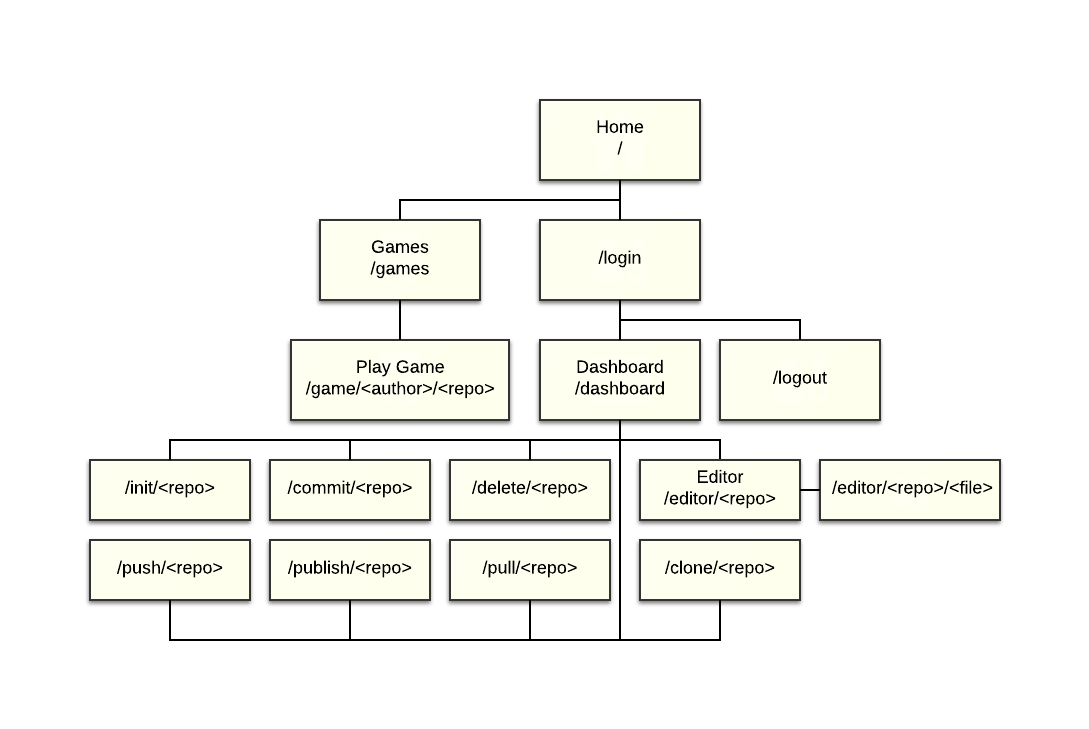
\includegraphics[scale=0.8]{webserverroutes}
		\caption{Web server routes}
		\label{fig:webserverroutes}
	\end{figure}

	\subsection{Game Engine}
	The game engine follows the Entity-Component-System architectural pattern and is separated into three major objects; \textbf{Scenes}, \textbf{Entities} and \textbf{Components}. These are the basis for the game engine structure, which is visualised in Figure \ref{fig:gameenginedesign}. A number of pre-defined components are designed to assist users in creating their games without having to make the low level building blocks of the game engine. These include the \emph{transform}, \emph{mesh}, \emph{camera}, \emph{light} and \emph{physics} components. New components can be created in the editor using JavaScript to add to the functionality of the game engine.

	% ref ECS design

	\begin{figure}[h]
		\centering
		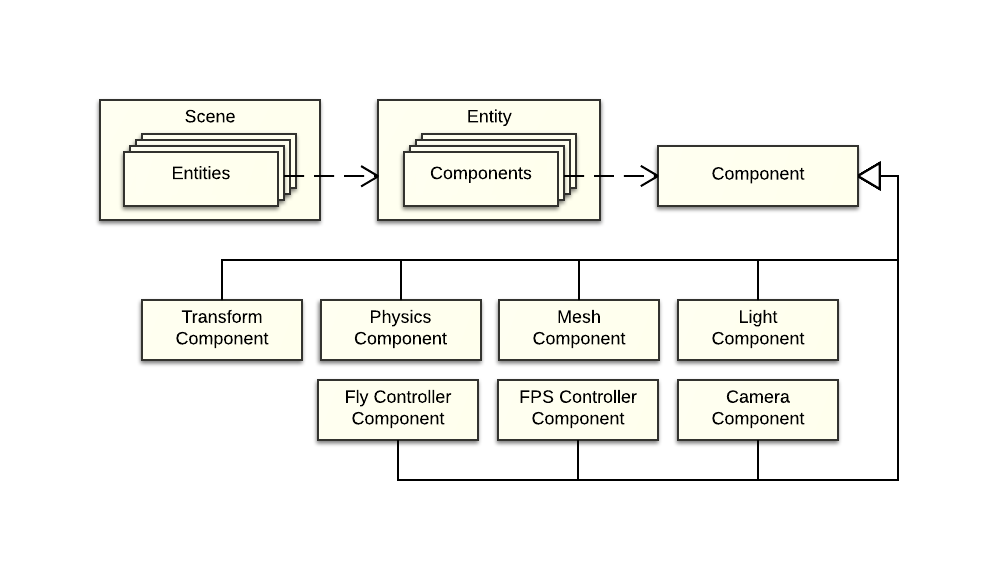
\includegraphics[scale=0.8]{gameenginedesign}
		\caption{Game engine structural design}
		\label{fig:gameenginedesign}
	\end{figure}

	\paragraph{File structure.}
	The file structure of a game created in the game engine is consistent for each game. A gamedata.json file is used to represent the Scene-Entity-Component structure in the JSON serialized format, with properties for the game engine, each entity and their components being stored. Custom components created in the editor are stored in the `components' folder.

	\subsection{Game Editor}
	The game editor is where users will be able to modify their game projects. The game's data, which is structured as a JSON object will be modified here and saved automatically whenever changes are made to the game. The user can create new components here, by creating a script and editing it with the built-in text editor.

	The editor is designed as several \emph{views} which work together. These views are responsible for handling their own HTML events and rendering, with each view being able to contain other views. This design allows the complex user interface to be built up in a modular way, by building more complicated views as a container of several smaller views.

	\paragraph{SceneView.}
	The central part of the editor, the scene view will be an implementation of the game engine. Changes to the list of scenes \& entities, or changing properties of a component will cause the view to update real-time. This provides the user with visual feedback when they make changes to their game. The Scene View will also display an indicator on the currently selected object, allowing them to move the object in 3D space by clicking and dragging one of the axes.

	\paragraph{Saving.}
	The game editor will automatically save any changes to the game every few seconds (If there were changes made). Any scripts the user is currently editing will also be saved, either every few seconds or when the script tab has been closed. Changes will also be saved if the user navigates away from the editor, or changes window; updating the game instantly if the user switches to playing the game tab in their browser.

\section{Use Cases \& Features}
A use case diagram was created to model the possible actions a user can take while accessing the system. Figure \ref{fig:usecasediagram} shows the use case diagram, which demonstrates the actions that a guest user may perform compared to a user who is logged in. The creation of this use case diagram assisted in solidifying the features that were required for this project, as it clearly defines the minimal amount of user actions needed in the system.

\begin{figure}[h]
	\centering
	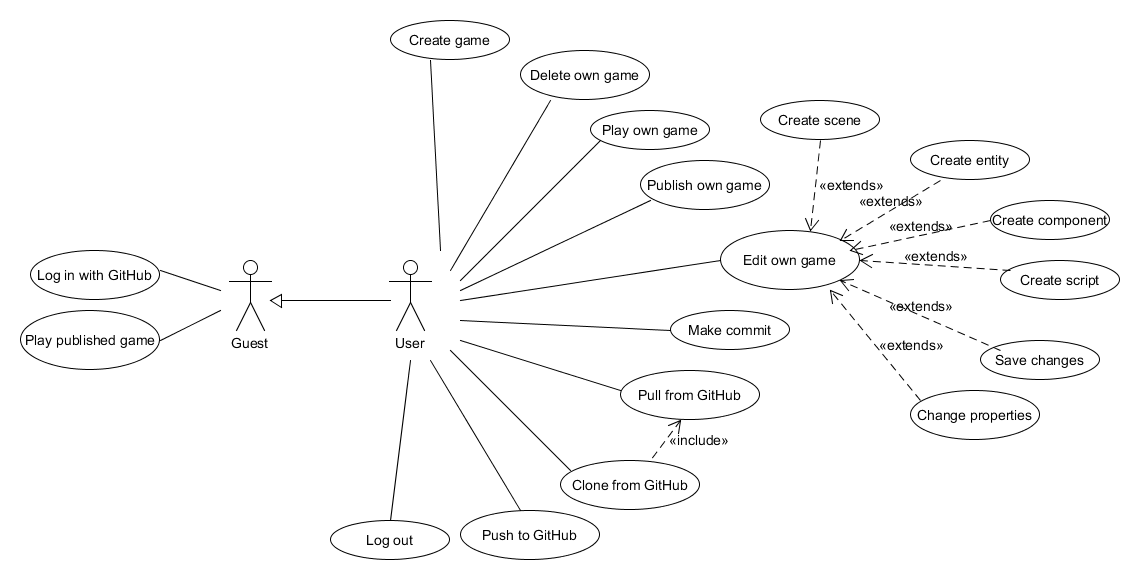
\includegraphics[scale=0.3]{use_case}
	\caption{Use case diagram}
	\label{fig:usecasediagram}
\end{figure}

The actions available to guest users are to either play a published game, or log in. When a guest logs into the system through GitHub they become a user, where they can perform several actions in addition to the actions a guest can perform. The actions a user can take are listed below:

\begin{itemize}
	\item Create a new game
	\item Delete one of their games
	\item Play their game
	\item Publish their game
	\item Edit their game:
	\begin{itemize}
		\item Add a scene
		\item Add an entity
		\item Add a component to an entity
		\item Change properties of an entity and it's components
		\item Create a new scripted component
		\item Save their changes
	\end{itemize}
	\item Commit changes to a game
	\item Pull from GitHub
	\item Push to GitHub
	\item Clone a game project from GitHub
	\item Log out
\end{itemize}

% todo: ********
% Clearly identify the list of features and use cases supported within the project